\appendix
\UnnumberedChapter{PHỤ LỤC}

% Đánh số hình/bảng trong phụ lục dạng PL.1, PL.2 (chương không đánh số nên không dùng số chương).
\renewcommand{\thetable}{PL.\arabic{table}}
\renewcommand{\thefigure}{PL.\arabic{figure}}
\setcounter{table}{0}\setcounter{figure}{0}

\section*{Phụ lục 1. Hướng dẫn tái lập kết quả}

\textbf{Yêu cầu:} Python $\ge3{,}10$. Môi trường nhóm dùng để sinh số liệu trong báo cáo: Python 3.14.6, scikit-learn 1.9.0, NumPy 2.4.1, pandas 3.1.0 (xem Bảng~\ref{tab:moi-truong}).

\begin{verbatim}
pip install -r requirements.txt

python -m spam_filter eda      # thống kê và biểu đồ EDA
python -m spam_filter run      # chạy E0..E6, lưu mô hình, bảng, lỗi
python -m spam_filter viz      # bộ biểu đồ cho báo cáo (viz_*.png)
python -m spam_filter viz --stability   # lặp 10 random_state
python -m spam_filter check    # kiểm tra rò rỉ / học thuộc / baseline
python -m spam_filter predict "Free entry! Call to win 500"
pytest                         # 41 kiểm thử
streamlit run app.py           # ứng dụng demo
\end{verbatim}

\textbf{Thứ tự khuyến nghị:} \texttt{eda} $\to$ \texttt{run} $\to$ \texttt{viz} $\to$ \texttt{check} $\to$ \texttt{streamlit run app.py}. Thư mục \texttt{outputs/} không được đưa lên git vì sinh lại được bằng các lệnh trên. Các hình trong thư mục \texttt{reports/images/} của báo cáo được sao chép từ \texttt{outputs/figures/}.

\textbf{Về phép đo độ nhạy (Bảng~\ref{tab:nhay}, \ref{tab:ablation}) và ngưỡng (Bảng~\ref{tab:nguong}).} Các bảng này được sinh bằng một đoạn mã tạm thời gọi lại chính các mô-đun của \texttt{spam\_filter} (\texttt{TextCleaner}, \texttt{build\_vectorizer}, \texttt{cross\_val\_f1}) với cùng cách chia dữ liệu và \texttt{random\_state}=42; đoạn mã này chưa được đưa vào kho mã nguồn dưới dạng lệnh CLI.

\textbf{Ghi chú về phiên bản.} Phiên bản README trước đây của dự án ghi E3 ROC-AUC 0,9682 và E5 CV F1 0,9414. Khi chạy lại với mã hiện tại, E3 cho 0,9685 và E5 cho 0,9425 (do bước nhận diện URL được cải tiến); báo cáo này dùng các số mới.

\section*{Phụ lục 2. Ma trận nhầm lẫn của mô hình E5}

\begin{figure}[H]
    \centering
    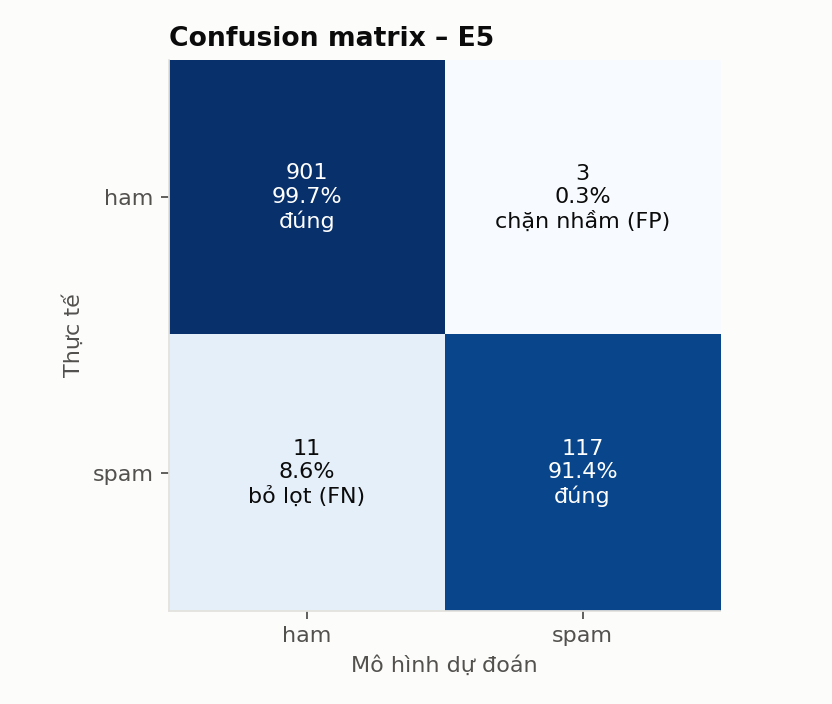
\includegraphics[width=0.6\textwidth]{images/viz_5_confusion_matrix.png}
    \caption{Ma trận nhầm lẫn của E5 trên tập kiểm tra (1\,032 tin)}
    \label{fig:cm-e5}
    \Nguon{Nhóm xây dựng từ kết quả thí nghiệm}
\end{figure}

\section*{Phụ lục 3. Khai báo sử dụng công cụ trí tuệ nhân tạo}

\begin{table}[H]
\centering
\caption{Khai báo sử dụng AI}
\label{tab:ai}
\small
\begin{tabular}{|>{\raggedright\arraybackslash}p{2.4cm}|>{\raggedright\arraybackslash}p{3.6cm}|>{\raggedright\arraybackslash}p{3.4cm}|>{\raggedright\arraybackslash}p{4cm}|}
\hline
\textbf{Công cụ} & \textbf{Mục đích} & \textbf{Phần liên quan} & \textbf{Nhóm đã kiểm tra/chỉnh sửa} \\
\hline
Claude Code & Dựng khung mã nguồn và hướng dẫn làm bài & Thư mục \texttt{spam\_filter/}, tệp \texttt{HUONG\_DAN\_} \texttt{LAM\_BAI.md} & \textit{(nhóm điền: cách kiểm tra, chạy lại và chỉnh sửa)} \\
\hline
Claude Code & Soạn thảo mã nguồn LaTeX của báo cáo từ kết quả thực nghiệm và mẫu báo cáo & Thư mục \texttt{reports/} & \textit{(nhóm điền: đối chiếu số liệu với \texttt{outputs/results/}, chỉnh sửa nội dung)} \\
\hline
\end{tabular}
\Nguon{Nhóm khai báo; xem thêm tệp \texttt{AI\_USAGE.md}}
\end{table}

\section*{Phụ lục 4. Phân công công việc}

\begin{table}[H]
\centering
\caption{Phân công công việc của nhóm}
\label{tab:phan-cong}
\begin{tabular}{|c|p{3.6cm}|p{4cm}|p{3.8cm}|}
\hline
\textbf{STT} & \textbf{Họ và tên} & \textbf{Mã sinh viên} & \textbf{Nhiệm vụ} \\
\hline
1 & \textit{(điền)} & \textit{(điền)} & \textit{(điền)} \\
\hline
2 & \textit{(điền)} & \textit{(điền)} & \textit{(điền)} \\
\hline
3 & \textit{(điền)} & \textit{(điền)} & \textit{(điền)} \\
\hline
\end{tabular}
\Nguon{Nhóm tổng hợp}
\end{table}
